\chapter{Thermal Convection Loop Experiment}
\chaptermark{Thermosyphon} %this is the chapter heading that will show on subsequent pages

\begin{quote}
The thermosyphon, a type of natural convection loop or non-mechanical heat pump, can be likened to a toy model of climate \shortcite{harris2011predicting}.
In this chapter we present both physical and computationally simulated thermosyphons, the equations governing their behavior, and results of the computational experiment.
\end{quote}

\section{Physical Thermal Convection Loops}

Under certain conditions, thermal convection loops operate as non-mechanical heat pumps, making them useful in many applications.
In Figure \ref{fig:thermosyphons} we see three such applications.
In solar hot water heaters, water is warmed using the sun's energy, resulting in a substantial energy savings in solar-rich areas.
Solar hot water thermosyphons, filled with either water or antifreeze, are used to transfer the solar energy into a hot water tank.
Geothermal systems rely on the Earth's warmth deep underground to heat and cool buildings, and due to low temperature differences are often augmented with a physical pump.
Cooling the CPU of modern computers is necessary for operation at high clock rate, and thermosyphons have been used to cool the CPU the while reducing noise and energy consumption.
The author notes the difference between forced and natural convection, where in some of these systems forced convection may be necessary in operation.

In response to a warming climate, thermosyphons have been used to transfer heat away from buildings built on fragile permafrost, which would otherwise melt and destroy the structure \shortcite{Xu2008experimental}.
These ground thermosyphons are pictured in Figure \ref{fig:fairbanks}.

\begin{figure}[h!]
  \centering
  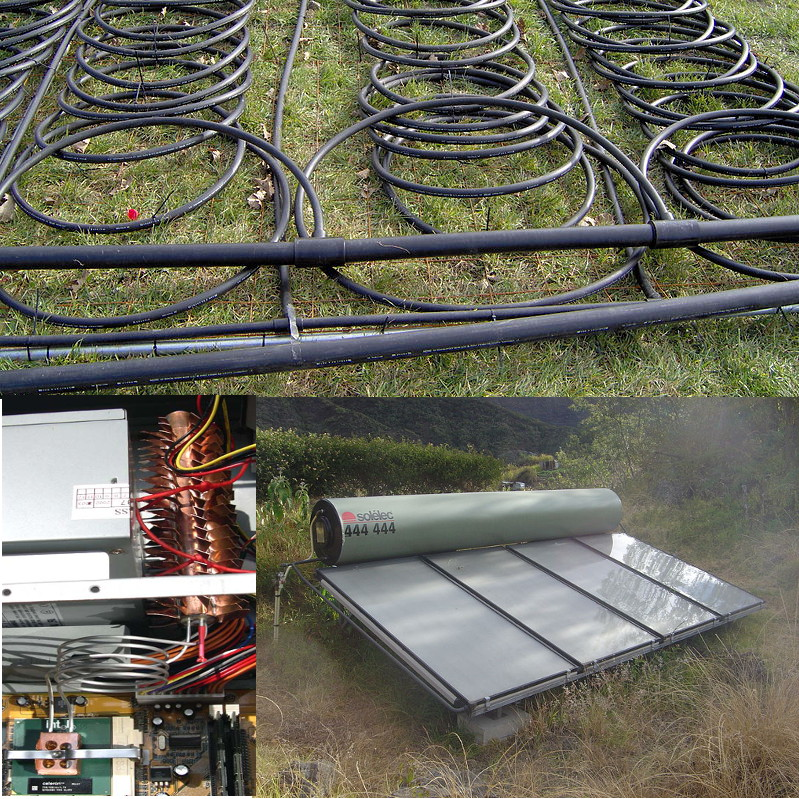
\includegraphics[width=0.89\textwidth]{figures/many-thermosyphons.jpg}
  \caption{
    Here we see many different thermosyphon applications.
    Clockwise starting at the top, we have a geothermal heat exchanger, solar hot water heater, and computer cooler. 
    Images credit to BTF Solar and Kuemel Bernhard {\protect\shortcite{CPUThermo,WSJthermo}}.
  }
  \label{fig:thermosyphons}
\end{figure}



\begin{figure}[b!]
  \centering
  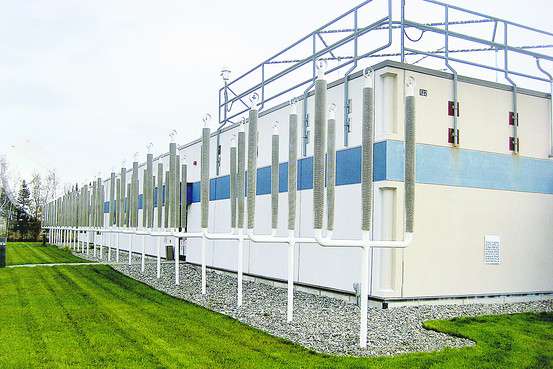
\includegraphics[width=0.79\textwidth]{figures/fairbanks-thermosyphon.jpg}
  \caption{
  Thermosyphons flank a Federal Aviation Administration building in Fairbanks, Alaska. 
  The devices help keep the permafrost frozen beneath buildings and infrastructure by transferring heat out of the ground.
  Photo credit Jim Carlton {\protect\shortcite{WSJthermo}}.    
  }
  \label{fig:fairbanks}
\end{figure}

\subsection{Ehrhard-M\"{u}ller Equations}

Following the derivation by Harris \shortcite{harris2011predicting}, itself a representation of the derivation of Gorman \shortcite{gorman1986} and namesakes Ehrhard and M\"{u}ller \shortcite{ehrhard1990dynamical}, we derive the equations governing a closed loop thermosyphon.

Similar to the derivation of the governing equations of computational fluid dynamics in Appendix B, we start with a small but finite volume inside the loop.
Here, however, the volume is described by $\pi r^2 R \text{d} \phi$ for $r$ the interior loop size (such that $\pi r^2$ is the area of a slice) and $R\text{d}\phi$ the arc length (width) of the slice.
Newton's second law states that momentum is conserved, such that the sum of the forces acting upon our finite volume is equal to the change in momentum of this volume.
Therefore we have the basic starting point for forces $\sum F$ and velocity $u$ as
\begin{equation} \sum F = \rho \pi r^2 R \text{d}\phi \diff{u}{t} .\end{equation}
The sum of the forces is $\sum F = F_{\{p,f,g\}}$ for net pressure, fluid shear, and gravity, respectively.
We write these as
\begin{align} & F_p = -\pi r^2 \text{d} \phi \pdiff{p}{\phi}\\
& F_w = -\rho \pi r^2 \text{d} \phi f_w\\
& F_g = -\rho \pi r^2 \text{d} \phi g \sin (\phi)\end{align}
where $\partial p /\partial \phi$ is the pressure gradient, $f_w$ is the wall friction force, and $g \sin (\phi)$ is the vertical component of gravity acting on the volume.

\begin{figure}[h!]
  \centering
  \includegraphics[width=0.79\textwidth]{../2013-05data-assimilation/papers/harris-tellus-2012-loop.pdf}
  \caption{
    Schematic of the experimental, and computational, setup from Harris et al (2012).
    The loop radius is given by $R$ and inner radius by $r$.
    The top temperature is labeled $T_c$ and bottom temperature $T_h$, gravity $g$ is defined downward, the angle $\phi$ is prescribed from the 6 o'clock position, and temperature difference $\Delta T_{3-9}$ is labeled.
  }
  \label{fig:thermosyphons}
\end{figure}

We now introduce the Boussinesq approximation which states that both variations in fluid density are linear in temperature $T$ and density variation is insignificant except when multiplied by gravity.
The consideration manifests as
\begin{equation*} \rho = \rho (T) \simeq \rho _\text{ref} (1 - \beta (T - T_\text{ref}) \end{equation*}
where $\rho _0$ is the reference density and $T_\text{ref}$ is the reference temperature, and $\beta$ is the thermal expansion coefficient.
The second consideration of the Boussinesq approximation allows us to replace $\rho$ with this $\rhoref$ in all terms except for $F_g$.
We now write momentum equation as
\begin{equation} -\pi r^2 \dphi \pdiff{p}{\phi} - \rhoref \phi r^2 R \dphi f_w
- \rhoref (1 - \rho (T- T_\text{ref}) ) \pi r^2 R \dphi g \sin (\phi) = \rhoref \pi r^2 R \dphi \diff{u}{t}. \end{equation}
Canceling the common $\pi r^2$, dividing by $R$, and pulling out $\dphi$ on the LHS we have
\begin{equation} -\dphi \left ( \pdiff{p}{\phi}  \frac{1}{R} - \rhoref f_w - \rhoref (1 - \rho (T- T_\text{ref}) ) g \sin (\phi) \right ) = \rhoref \dphi \diff{u}{t}. \label{eq:EM07} \end{equation}
We integrate this equation over $\phi$ to eliminate many of the terms, specifically we have
\begin{align*}
& \int _{0} ^{2\pi} -\dphi \pdiff{p}{\phi} \frac{1}{R} \rightarrow 0\\
& \int _{0} ^{2\pi} -\dphi \rhoref g \sin (\phi) \rightarrow 0\\
& \int _{0} ^{2\pi} -\dphi \rhoref \beta T_\text{ref} g \sin (\phi) \rightarrow 0.\end{align*}
Since $u$ (and hence $\diff{u}{\phi}$) and $f_w$ do not depend on $\phi$, we can pull these outside an integral over $\phi$ and therefore the momentum equation is now 
\begin{equation*} 2\pi f_w \rho _0 + \int _{0} ^{2\pi} \dphi \rhoref \beta T g \sin (\phi) = 2\pi \diff{u}{\phi} \rhoref .\end{equation*}
Diving out $2\pi$ and pull constants out of the integral we have our final form of the momentum equation
\begin{equation} f_w \rhoref + \frac{\rhoref \beta g }{2 \pi} \int _{0} ^{2\pi} \dphi T \sin (\phi) = \diff{u}{\phi} \rhoref \label{eq:EM10}.\end{equation}
Now considering the conservation of energy within the thermosyphon, the energy change within a finite volume must be balanced by transfer within the thermosyphon and to the walls.
The internal energy change is given by
\begin{equation} \rhoref \pi r^2 R \dphi \left ( \pdiff{T}{t} + \frac{u}{R}\pdiff{T}{\phi} \right ) \label{eq:EMeg1}\end{equation}
which must equal the energy transfer through the wall, which is, for $T_w$ the wall temperature:
\begin{equation} \dot{q} = -\pi r^2 R \dphi h_w (T - T_w) . \label{eq:EMeg2} \end{equation}
Combining Equations \ref{eq:EMeg1} and \ref{eq:EMeg2} (and canceling terms) we have the energy equation:
\begin{equation} \left ( \pdiff{T}{t} + \frac{u}{R}\pdiff{T}{\phi} \right ) = \frac{-h_w}{\rhoref c_p} \left( T - T_w \right ) \label{eq:EMeq}.\end{equation}
The $f_w$ which we have yet to define and $h_w$ are fluid-wall coefficients and can be described by \shortcite{ehrhard1990dynamical}:
\begin{align*} & h_w = h_{w_0} \left ( 1 + K h(|x_1|) \right ) \\
& f_w = \frac{1}{2} \rhoref f_{w_0} u .\end{align*}
We have introduced an additional function $h$ to describe the behavior of the dimensionless velocity $x_1 \alpha u$.
This function is defined piece-wise as 
\begin{equation*} h (x) = \left \{ \begin{array}{ll} x^{1/3} & ~~\text{when} ~x \geq 1\\ p (x) & ~~\text{when} ~ x <1 \end{array} \right. \end{equation*} 
where $p(x)$ can be defined as $p(x) = \left( 44x^2 -55 x^3 + 20x^4 \right ) /9$ such that $p$ is analytic at 0 \shortcite{harris2011predicting}.

Taking the lowest modes of a Fourier expansion for $T$ for an approximate solution, we consider:
\begin{equation} T(\phi , t) = C_0 (t) + S(t) \sin (\phi ) + C(t) \cos (\phi) . \end{equation}
By substituting this form into Equations \ref{eq:EM10} and \ref{eq:EMeq} and integrating, we obtain a system of three equations for our solution.
We then follow the particular nondimensionalization choice of Harris et al such that we obtain the following ODE system, which we refer to as the Ehrhard-M\"{u}ller equations:
\begin{align}
& \diff{x_1}{t'} = \alpha (x_2 - x_1),\\
& \diff{x_2}{t'} = \beta x_1 - x_2 (1 + Kh(|x_1|)) - x_1x_3,\\
& \diff{x_3}{t'} = x_1x_2 - x_3 (1 + Kh(|x_1|)) .\end{align}
The nondimensionalization is given by the change of variables
\begin{align}
& t' = \frac{h_{w_0}}{\rhoref c_p}t,\\
& x_1 = \frac{\rhoref c_p }{R h_{w_0}} u, \\
& x_2 = \frac{1}{2} \frac{\rhoref c_p \beta g}{ R h_{w_0} f_{w_0}} \Delta T_{3-9}, \\
& x_3 = \frac{1}{2} \frac{\rhoref c_p \beta g}{ R h_{w_0} f_{w_0}} \left ( \frac{4}{\pi} \Delta T_w - \Delta T_{6-12} \right ) 
\end{align}
and
\begin{align}
& \alpha = \frac{1}{2} R c_p f_{w_0} / h_{w_0} ,\\
& \gamma = \frac{2}{\pi} \frac{\rhoref c_p \beta g}{Rh_{w_0} f_{w_0}} \Delta T_w. \end{align}

Through careful consideration of these non-dimensional variable transformations we verify that $x_1$ is representative of the mean fluid velocity, $x_2$ of the temperature difference between the 3 and 9 o'clock positions on the thermosyphon, and $x_3$ the deviation from the vertical temperature profile in a conduction state \shortcite{harris2011predicting}.

\subsection{Experimental Setup}
Originally built (and subsequently melted) by Dr. Chris Danforth at Bates College, the University of Vermont's current experimental thermosyphons have made considerable progress.
Operated by Dave Hammond, UVM's Scientific Electronics Technician, the experimental thermosyphons access the chaotic regime of state space found in the principled governing equations.

\begin{figure}[h!]
  \centering
  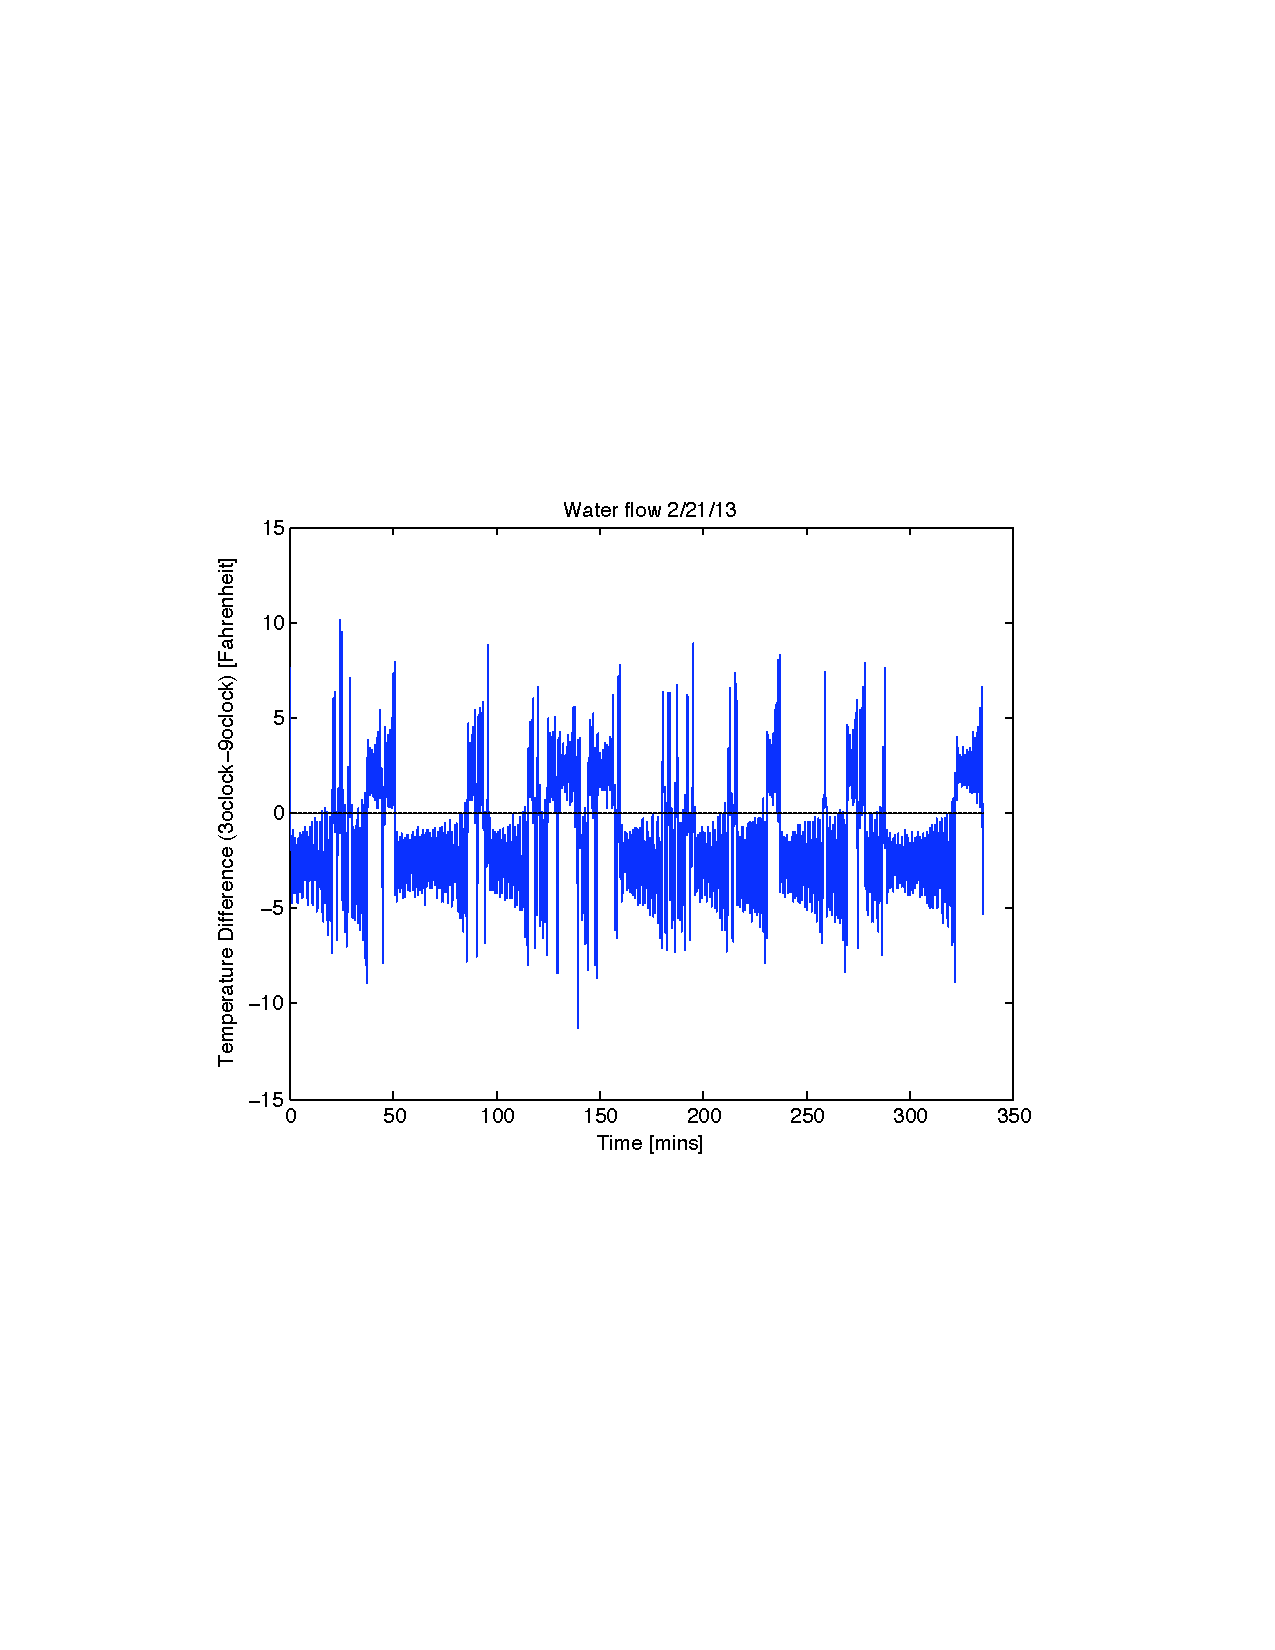
\includegraphics[width=0.95\textwidth]{figures/221TimeSeries.pdf}
  \caption{
    A time series of the physical thermosyphon, from the Undergraduate Honor's Thesis of Darcy Glenn {\protect \shortcite{glenn2013}}.
    The temperature difference (plotted) is taken as the difference between temperature sensors in the 3 and 9 o'clock positions.
    The sign of the temperature difference indicates the flow direction, where positive values are clockwise flow.
  }
  \label{fig:chrisLoop}
\end{figure}

\begin{figure}[h!]
  \centering
  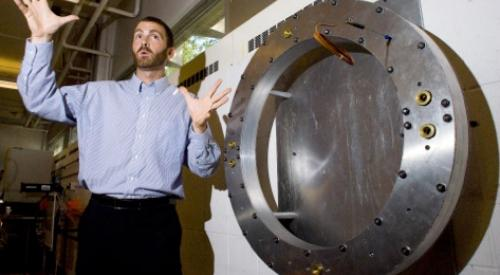
\includegraphics[width=0.49\textwidth]{figures/danforth.jpg}
  \caption{
  Professor Chris Danforth with the Thermal Convection Loop.
  Photo credit Tim Johnson, Burlington Free Press {\protect\shortcite{danforthFP}}.
  }
  \label{fig:chrisLoop}
\end{figure}


\section{Computational Experiment}
In this section, we first present the governing equations for the flow in our thermal convection loop experiment.
A spatial and temporal discretization of the governing equations is then necessary so that they may be solved numerically.
After discretization, we must specify the boundary conditions.
With the mesh and boundary conditions in place, we can then simulate the flow with a computational fluid dynamics solver.

We now discuss the equations, mesh, boundary conditions, and solver in more detail.
With these considerations, we present our simulations of the thermosyphon.

\subsection{Governing Equations}
We consider the incompressible Navier-Stokes equations with the Boussinesq approximation to model the flow of water inside a thermal convection loop.
Here we present the main equations that are solved numerically, noting the assumptions that were necessary in their derivation.
In Appendix B a more complete derivation of the equations governing the fluid flow, and the numerical for our problem, is presented.
In standard notation, for $u,v,w$ the velocity in the $x,y,z$ direction, respectively, the continuity equation for an incompressible fluid is
\begin{equation} \frac{\partial u}{\partial x} + \frac{\partial v}{\partial y} + \frac{\partial w}{\partial z} = 0. \label{eq:NScontIco} \end{equation}

The momentum equations, presented compactly in tensor notation, are given by
\begin{equation} \rho _0 \left ( \frac{\partial \bar{u}_i}{\partial t} + \frac{\partial}{\partial x_j} \left( \bar{u}_j \bar{u}_i \right) \right )
= -\frac{\partial \bar{p}} {\partial{x_i}} +  \mu \frac{\partial \bar{u}_i}{\partial x_j^2} + \bar{\rho} g_i. \end{equation}
%% \begin{equation*} g_i\frac{\bar{\rho}}{\rho _0} = g_i \left ( 1 + \frac{\bar{\rho} - \rho _0}{\rho _0} \right ) = g_i \rho _k  = g_i \left (1 - \beta \left (\overline{T} - T _0\right ) \right ) .\end{equation*}

Note that $g_i = 0$ for $i \in \{ x,y\}$ since gravity is assumed to be the $z$ direction.
The energy equation is given by

\begin{equation} \frac{\partial }{\partial t} \left ( \rho \overline{e}\right ) + \frac{\partial}{\partial x_j} \left ( \rho \overline{e} \overline{u}_j \right ) 
= 
- \frac{\partial q_k^*}{\partial x_k}
- \frac{\partial \overline{q}_k}{\partial x_k}.
\end{equation}

\subsection{Mesh}

Creating a suitable mesh is necessary to make an accurate simulation.
Both 2-dimensional and 3-dimensional meshes were created using OpenFOAM's native meshing utility ``blockMesh.''
After creating a mesh, we consider refining the mesh near the walls to capture boundary layer phenomena and renumbering the mesh for solving speed.
To refine the mesh near walls, we used the ``refineWallMesh'' utility, 
Lastly, the mesh is renumbered using the ``renumberMesh'' utility, which implements the Cuthill-McKee algorithm to minimize the adjacency matrix bandwidth, defined as the maximum distance from diagonal of nonzero entry.
The 2D mesh contains 40,000 points, and is imposed with fixed value boundary conditions on the top and bottom of the loop.

\begin{figure}[h!]
  \centering
  \includegraphics[width=0.79\textwidth]{/Users/andyreagan/work/2013/2013-05data-assimilation/OpenFOAM/figures/heating_zoom_mesh4.png}
  \caption{
  A snapshot of the mesh used for CFD simulations.
  Shown is an initial stage of heating for a fixed value boundary condition, 2D, laminar simulation with a mesh of 40000 cells including wall refinement with walls heated at 340K on the bottom half and cooled to 290K on the top half.
  }
  \label{fig:CFDmesh1}
\end{figure}

\begin{figure}[h!]
  \centering
  \includegraphics[width=0.79\textwidth]{/Users/andyreagan/work/2013/2013-05data-assimilation/OpenFOAM/figures/3D-mesh2.png}
  \caption{
  The 3D mesh viewed as a wireframe from within.
  Here there are 900 cells in each slice (not shown), for a total mesh size of 81,000 cells.
  Simulations using this computational mesh are prohibitively expensive for use in a real time ensemble forecasting system, but are possible offline.
  }
  \label{fig:CFDmesh2}
\end{figure}

\begin{figure}[h!]
  \centering
  \includegraphics[width=0.79\textwidth]{/Users/andyreagan/work/2013/2013-05data-assimilation/OpenFOAM/figures/adjacency36000bool01.pdf}
  \caption{
  The 2D mesh Adjacency matrix for a local radius of 1.0cm.
  In general, we see that cells have neighbors with nearby cell ID.
  With 5,260,080 nonzero entries, it is difficult to see structure looking at the entire matrix.
  }
  \label{fig:CFDmeshAdj1}
\end{figure}

\begin{figure}[h!]
  \centering
  \includegraphics[width=0.79\textwidth]{/Users/andyreagan/work/2013/2013-05data-assimilation/OpenFOAM/figures/adjacency36000bool02.pdf}
  \caption{
  The 2D mesh adjacency matrix, zoomed in.
  The Cuthill-McKee renumbering algorithm was used, and we see 23 distinct regions of local numbering, reflective of the geometry and Cuthill-McKee algorithm.
  The mesh shown here has 30 cells in each perpendicular slice of the loop, and they are numbered iteratively along the edge of triangular front emanating from cell 0 (chose to be the left-most cell).
  This diagonalization in both space and ID number effectively reduces the bandwidth of the mesh from 947 to 18.
    }
  \label{fig:CFDmeshAdj2}
\end{figure}

\subsection{Boundary Conditions}

Available boundary conditions (BCs) that were found to be stable in OpenFOAM's solver were constant gradient, fixed value conditions, and turbulent heat flux.
Simulations with a fixed flux BC is implemented through the externalWallHeatFluxTemperature library were unstable and resulted in physically unrealistic results.
Constant gradient simulations were stable, but the behavior was empirically different from our physical system.
Results from attempts at implementing these various boundary conditions are presented in Table \ref{tb:ofbc}.
To most accurately model our experiment, we choose a fixed value BC.
This is due to the thermal diffusivity and thickness of the walls of the experimental setup.
For $Q$ the flow of heat from the hot water bath into the loop's outer material, and $A$ the area of a small section of boundary we can write the heat flux $q$ into the fluid inside the loop as a function of the thermal conductivity $k$, temperature difference $\Delta T$ and wall thickness $\Delta x$:
\begin{equation} q = \frac{Q}{A} = k \frac{\Delta T}{\Delta x} . \end{equation}
For our experimental setup, the thermal conductivity of a PVC wall is approximately $1.1 \, \left [ \text{BTU in}/(h\cdot \text{ft}^2 F) \right ]  = 0.15 \, \left [W/(m\cdot K)\right ] $.
With a wall thickness of 1cm, and $\Delta T = 10 \left [K \right ]$ the heat flux is $q=79 \left [ W/m^2 \right ]$.
The numerical implementation of this boundary condition is considered further in Appendix D.
In Table \ref{tb:ofbc} we list the boundaries conditions with which we experimented, and the quality of the resulting simulation.

\begin{table}
\begin{tabular}{llll}
\hline
Boundary Condition & Type & Values Considered & Result\\
\hline
\hline
fixedValue & value & $\pm 5 \to \pm 30$ & realistic\\
\hline
fixedGradient & gradient & $\pm 10 \to \pm 100000$ & plausible\\
\hline
wallHeatTransfer & enthalpy & - & cannot compile\\
\hline
externalWallHeatFluxTemperature & flux & - & cannot compile\\
\hline
turbulentHeatFluxTemperature & flux & $\pm .001 \to \pm10$ & unrealistic\\
\hline
\end{tabular}
\label{tb:ofbc}
\caption{
  Boundary conditions considered for the OpenFOAM CFD model are labeled with their type, values considered, and empirical result.
  We find the most physically realistic simulations using the simplest ``fixedValue'' condition.
  The most complex conditions, ``wallHeatTransfer,'' ``externalWallHeatFluxTemperature,'' and ``turbulentHeatFluxTemperature'' either did not compile or produced divergent results.
  }
\end{table}

\subsection{Solver}

In general, there are three approaches to the numerical solution of PDEs: finite differences, finite elements, and finite volumes.
We perform our computational fluid dynamics simulation of the thermosyphon using the open-source software OpenFOAM.
OpenFOAM has the capacity for each scheme, and for our problem with an unstructured mesh, the finite volume method is the simplest.
The solver in OpenFOAM that we use, with some modification, is ``buoyantBoussinesqPimpleFoam.''
Solving is accomplished by the Pressure-Implicit Split Operator (PISO) algorithm \shortcite{issa1986solution}.
Modification of the code was necessary for laminar operation.
In Table \ref{tb:ofsolution}, we note the choices of schemes for time-stepping, numerical methods and interpolation.

%% Links for OpenFOAM code documentation:
%% \url{http://www.openfoam.org/docs/user/compiling-applications.php}
%% \url{http://www.openfoam.org/docs/cpp/}

The Boussinesq approximation makes the assumption that density changes due to temperature differences are sufficiently small so that they can be neglected without effecting the flow, except when multiplied by gravity.
The non-dimensionalized density difference $\Delta \rho / \rho$ depends on the value of heat flux into the loop, but remains small even for large values of flux.
Below, we approximate the validity of the Boussinesq approxmaintion, which is generally valid for values of $\beta(T-T_\text{ref})\rhoref \ll 1$:
\begin{equation} \frac{\beta(T - T_\text{ref})}{\rhoref} \simeq 7.6 \cdot 10^{-6} \ll 1 \label{eq:bouss} \end{equation}

\begin{table*}
\begin{center}
\begin{tabular}{ll}
\hline
Problem & Scheme\\
\hline
\hline
Main solver & buoyantBoussinesqPimpleFoam\\
\hline
Solving algorithm & PISO\\
\hline
Grid & Semi-staggered\\
\hline
Turbulence model & None (laminar)\\
\hline
Time stepping & Euler\\
\hline
Gradient & Gauss linear\\
\hline
Divergence & Gauss upwind\\
\hline
Laplacian & Gauss linear\\
\hline
Interpolation & Linear\\
\hline
Matrix preconditioner & Diagonal LU\\
\hline
Matrix solver & Preconditioned Bi-linear Conjugate Gradient\\
\hline
\end{tabular}
\caption{
  Numerical schemes used for solving the finite volume problem.
  }
\label{tb:ofsolution}
\end{center}
\end{table*}

\subsection{Simulation results}
With the mesh, BCs, and solver chosen, we now simulate the flow.
From the data of $T,\phi,u,v,w$ and $p$ that are saved at each timestep, we extract the mass flow rate and average temperature at the $12,3,6$ and $9$ o'clock positions on the loop.
Since $\phi$ is saved as a face-value flux, we compute the mass flow rate over the cells $i$ of top (12 o'clock) slice as
\begin{equation} \sum _i\phi_{f(i)} \cdot v_i \cdot \rho_i\end{equation}
where $f(i)$ corresponds the face perpendicular to the loop angle at cell $i$ and $\rho$ is reconstructed from the Boussinesq approximation $\rho = \rhoref (1-\beta(T-T_\text{ref}))$.

Here is a picture of the thermosyphon colored by temperature.
\begin{figure}[h!]
  \centering
  \includegraphics[width=0.95\textwidth]{/Users/andyreagan/work/2013/2013-05data-assimilation/OpenFOAM/figures/heating003.png}
  \caption{
  A screenshot of the whole loop.
  Shown is an initial stage of heating for a fixed value boundary condition, 2D, laminar simulation with a mesh of 40000 cells including wall refinement with walls heated at 340K on the bottom half and cooled to 290K on the top half.
  }
  \label{fig:CFDloopSS}
\end{figure}






















